%%%%%%%%%%%%%%%%%%%%%%%%%%%%%%%%%%%%%%%%%%%%%%%%%%%%%%%
%%%%% Sec: Lens reconstruction  %%%%%
%%%%%%%%%%%%%%%%%%%%%%%%%%%%%%%%%%%%%%%%%%%%%%%%%%%%%%%
\section{Lens reconstruction}
\label{sec:lens_reconstruction}

One of the primary applications of gravitational lensing is reconstructing the lens mass distribution. The modeling of gravitational lenses begins with a collection of observables (\cref{fig:observables}), such as the relative positions and fluxes of images, time delays between images, and other properties of the lens. This modeling can be approached in one of two different but related ways: as a \emph{forward} problem of creating a model of the lens system (lenses and sources) that approximates the observed image the best, or as the \emph{inverse} problem of finding a lens model that deconstructs the observation into a self-consistent and physically viable image of the source. Many successful applications have been published for both the forward \citep{bandara_witnessing_2013,bolton_sloan_2008,newton_sloan_2011,peng_probing_2006} and the inverse method \citep{dye_decomposition_2005,kochanek_lensclean_1992,nightingale_adaptive_2015,suyu_bayesian_2006,vegetti_bayesian_2009,wallington_lensmem_1996,warren_semilinear_2003}.

\begin{figure}
    \centering
    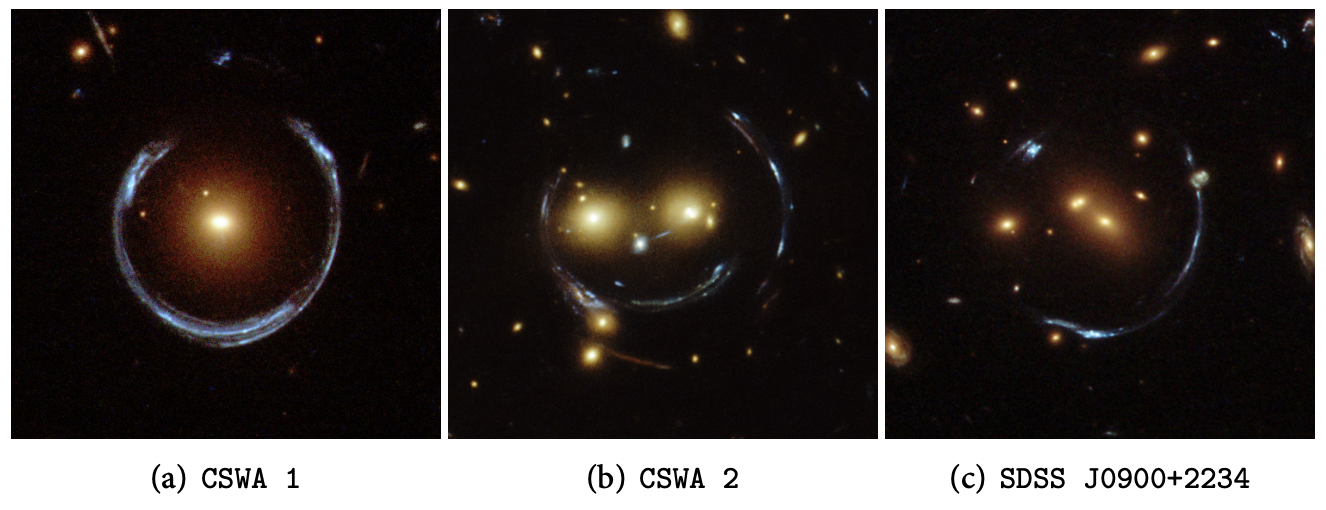
\includegraphics[width=\linewidth, keepaspectratio]{img//chapter4/observables.png}
    \caption[Strong gravitational lensing observations]{Examples of observations of strong gravitational lensing. The large arcs contain information to constrain the gravitational lenses producing these images. \small{Credits: ESA/Hubble $\&$ Nasa}.}
    \label{fig:observables}
\end{figure}

Three types of constraints can be used for this purpose:
\begin{enumerate}
    \item the locations of the multiple images produced by a lensed source help to map out the deflection field of the lens, which corresponds to the first derivatives of the lensing potential \citep{cardone_gravitational_2001}. Obtaining these constraints is relatively straightforward assuming the availability of high-resolution imaging data. This work will mainly focus on this type of constraint.
    \item the magnifications (fluxes) and shapes of the multiple images and gravitational arcs explore the higher-order derivatives (mainly the second) of the lensing potential \citep{gilman_probing_2019}. Therefore, these constraints are particularly sensitive to the smaller-scale mass components of the lens;
    \item the relative time delays between multiple images serve as probes of the lensing potential, as shown in \cref{subsec:time_delay_images}. However, time delays can only be measured in a limited number of lenses (only a few tens) because they require the lensed sources to be intrinsically variable, such as quasars or supernovae \citep{refsdal_possibility_1964}. These types of source are rare. Additionally, measuring time delays is challenging; it demands dedicated telescope time for the continuous observation of these sources over extended periods, along with precise photometry.
\end{enumerate}

The method of translating observed strong lensing constraints into distributions of matter is referred to as lens \emph{inversion} or \emph{reconstruction}.

Such reconstruction is often tackled using two main categories of inversion algorithms \emph{parametric} and \emph{non-parametric} algorithms, based on whether the calculation is ``model-based'' (parametric) or ``model-free'' (non-parametric) at the start of the process \citep{coe_lensperfect_2008}. This work is focused on the first type of approach, applying parametric optimization to retrieve the mass distribution of the lens.

Each approach has its own particular set of strengths and weaknesses, which are summarized here.
\begin{enumerate}

    \item Parametric models employ a clear physical parameterization from the beginning, defining the mass distribution based on a set of specific parameters. Parametric simulation models are generally used to solve the forward problem, taking a source and lensing mass and then predicting the resulting image. Also known as simply-parameterized models, they assume a physical model that fits the data with relatively few defined parameters \citep{jullo_bayesian_2007}. In parametric models, the data is fitted to a physical object (\eg Point-Mass, Singular Isothermal Sphere, Singular Isothermal Ellipsoid, De Vaucouleurs model, etc.) and a model of the lensing mass made using that physical object to predict the effect on the light from the source, often with the assumption that mass follows light. The exploration of these models parameter space aims to identify the optimal combination that accurately replicates the observed positions, shapes, magnitudes, and relative time delays of the multiple images and arcs;

    \item non-parametric methods, which do not start with a predefined physical model but instead use a ``grid-based'' approach, among others, to model the mass distribution. The lens is divided into a mesh, which can be either structured or unstructured, and the lensing observables are projected onto this mesh. Subsequently, this mesh is converted into a pixelized mass distribution using the relationships between the observables and the surface density of the lens. This technique has been extensively applied on a variety of scales, from galaxies to clusters, and has been implemented in numerous ways \citep{birrer_gravitational_2015,blandford_modeling_2000,coles_gravitational_2014,diego_non-parametric_2005,diego_combined_2007,koopmans_gravitational_2005,liesenborgs_genetic_2006,merten_mesh-free_2016,saha_portable_2004,sebesta_testing_2016,suyu_anatomy_2006,suyu_dissecting_2009}.
\end{enumerate}


%%%%%%%%%%%%%%%%%%%%%%%%%%%%%%%%%%%%%%%%%%%%%%%%%%%%%%%
%%%%% SubSec: Parametric reconstruction %%%%%
%%%%%%%%%%%%%%%%%%%%%%%%%%%%%%%%%%%%%%%%%%%%%%%%%%%%%%%
\subsection{Parametric reconstruction}
\label{subsec:parametric_reconstruction}
Strong lensing parametric reconstruction, also known as inversion, involves the use of predefined models to describe both the mass distribution of the lensing object and the light distribution of the background source. The aim is to adjust the parameters of these models to best fit the observed lensing phenomena, such as arcs, rings, and multiple images of a background source. The process is detailed and involves several key steps and algorithms:
\begin{enumerate}
    \item \textbf{model selection} for both the mass distribution and the light distribution;
    \item \textbf{parameter initialization} for the parameters of the mass and light distribution models are made based on observational data or theoretical considerations;
    \item \textbf{ray-tracing simulation} using the initial models: a ray-tracing algorithm computes the deflection angles at each point in the lens plane, which are used to trace the light rays back to the source plane. This step predicts the appearance of the lensed images based on the current model parameters;
    \item \textbf{optimization} via an objective (loss) function that quantifies the difference between the observed and predicted lensed images, as described in \cref{sec:diff_prog}. This function often includes terms for the positions, shapes, and flux ratios of the observed and model-predicted images. Methods such as gradient descent \citep{ruder_overview_2016,canu_introduction_2016}, Markov Chain Monte Carlo (MCMC) \citep{geyer_practical_1992,speagle_conceptual_2019}, or Nested-Sampling \citep{skilling_nested_2004,buchner_nested_2023} are used to adjust model parameters to minimize the objective function. This iterative process refines the model to better fit the observations;
    \item \textbf{model comparison and selection} if multiple models are being tested, and statistical criteria such as the Akaike Information Criterion (AIC) \citep{cavanaugh_akaike_2019} or Bayesian Information Criterion (BIC) \citep{liddle_information_2007,chen_extended_2008} are used to compare their fit to the data, helping to select the best model;
    \item \textbf{uncertainty quantification} for the model parameters, often through bootstrapping or by analyzing the posterior probability distributions in methods like MCMC, providing insights into the confidence levels of the mass and light distribution parameters.
\end{enumerate}

As already stated, parametric reconstruction is highly dependent on the chosen models and their ability to accurately represent the complex mass distributions of astronomical objects. Its strength lies in its relatively straightforward interpretation and the physical significance of the model parameters, but it also faces limitations in flexibility compared to non-parametric methods.

There are several ways to implement parametric lens reconstruction and, as will be shown in \cref{chap:applications}, one of the most common approaches is to use the observed positions of multiple images (\cref{fig:multiple_images_param}).
The optimization can then be performed in mainly two ways: with the so-called \emph{lens} or \emph{image plane optimization} or with the \emph{source plane optimization} technique.

\begin{figure}
    \centering
    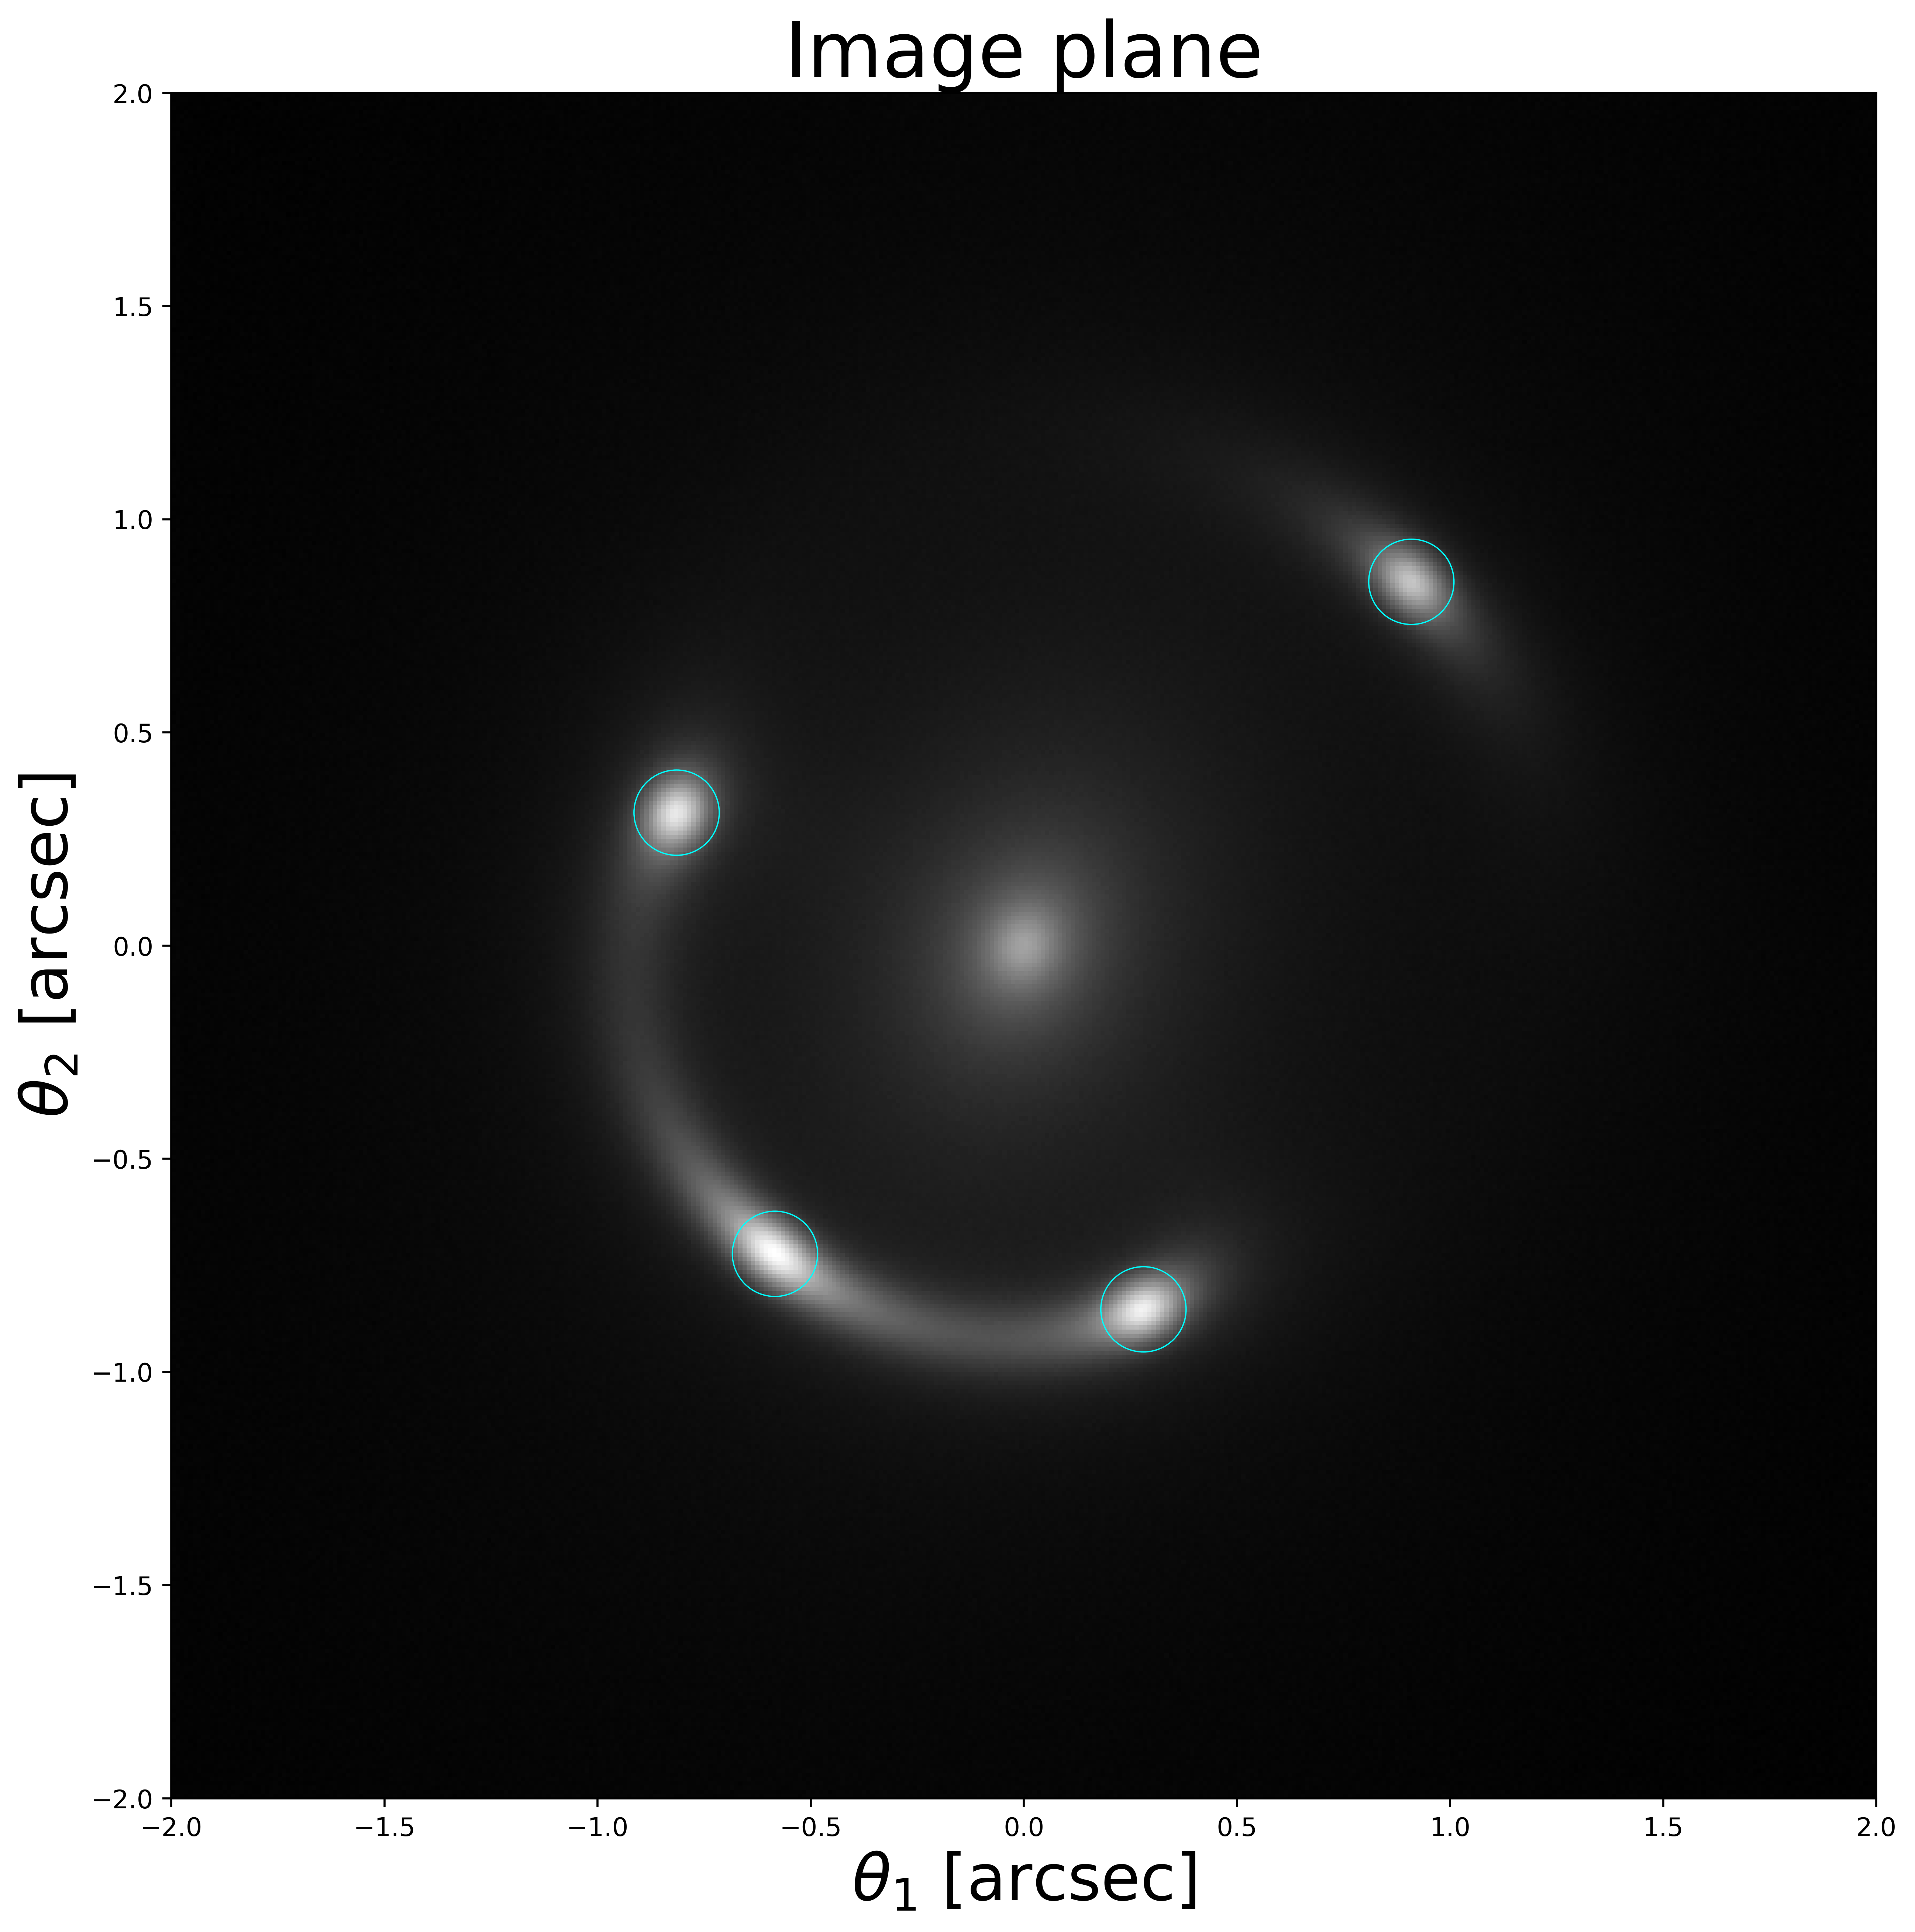
\includegraphics[width=0.6\linewidth, keepaspectratio]{img//chapter4/multiple_images_param.png}
    \caption[Simulated image of a strong lensing event with multiple images]{Simulated image of a strong lensing event with multiple images, indentified by the azure circles. The image is $\SI{4}{\arcsecond} \times \SI{4}{\arcsecond}$, with a pixel scale of $\SI{0.03}{\arcsecond}$.}
    \label{fig:multiple_images_param}
\end{figure}

%%%%%%%%%%%%%%%%%%%%%%%%%%%%%%%%%%%%%%%%%%%%%%%%%%%%%%%
%%%%% SubSubSec: Lens plane and source plane optimization %%%%%
%%%%%%%%%%%%%%%%%%%%%%%%%%%%%%%%%%%%%%%%%%%%%%%%%%%%%%%
\subsubsection{Lens plane and source plane optimization}
\label{subsubsec:lens_plane_source_plane_optimization}
In the context of lens inversion, the positions of multiple images $\va{\t}_i$ are the main observable feature that can be used to constrain the lens parameters. It is assumed that the lens is described by a surface density model (\eg SIS, SIE, etc.) depending on a set of $n$ parameters $\vec{p} = [p_1, \ldots, p_n]$, starting at some initial values (random or constrained by other observables) and that the redshifts of the source and lens are known.

\begin{itemize}
    \item \textbf{Lens plane optimization}

    Given a set of lens parameters, it is possible to calculate the lens deflection angle at the observed positions of the images $\va{\a} (\va{\t}_i | \vec{p})$ and, using the lens equation, map these positions on the source plane:
    \be
    \label{eq:4.19}
    \va{\b}_i (\vec{p}) = \va{\t}_i - \va{\a} ( \va{\t}_i | \vec{p}) \,.
    \ee

    The resulting points $\va{\b}_i (\vec{p})$ will be spread over a certain region in the source plane since the model parameters are not correct. The predicted source position can be estimated by taking the mean position of these points:
    \be
    \label{eq:4.20}
    \va{\b} (\vec{p}) = \frac{1}{N_{ima}} \sum\limits_{i=1}^{N_{ima}} \va{\b}_i (\vec{p}) \,,
    \ee
    where $N_{ima}$ is the observed number of multiple images.

    Subsequently, by solving the lens equation, the predicted source position can be mapped back to the lens plane, obtaining a set of predicted image positions
    \be
    \label{eq:4.21}
    \va{\b} (\vec{p}) \rightarrow \{\va{\t}_i (\vec{p}) ; i = 1, \ldots, N_{ima, \vec{p}}\} \,,
    \ee
    where the number of predicted images, $N_{ima, \vec{p}}$, can clearly be different from $N_{ima}$.

    At this point a cost function can be defined to compare the predicted and observed positions of the images
    \be
    \label{eq:4.22}
    \chi^2 (\vec{p}) = \sum\limits_{i=1}^{N_{ima}} \frac{[\va{\t}_i - \va{\t}_i (\vec{p})]^2}{\s_i^2} \,,
    \ee
    where $\va{\t}_i (\vec{p})$ is the position of the predicted image closest to the image at $\va{\t}_i$ and $\s_i$ is the error on the position of the $i$-th image.

    To identify the optimal lens model, one can adjust the parameters $\vec{p}$ to minimize the loss function, or equivalently, to maximize the likelihood of the observed image positions given the parameters $\vec{p}$
    \be
    \label{eq:4.23}
    \mathscr{L} (\vec{p}) = \frac{1}{\prod\limits_{i=1}^{N_{ima}} \s_i \sqrt{2 \pi}} \exp \left[ - \frac{\chi^2 (\vec{p})}{2} \right] \,.
    \ee

    When dealing with multiple families of multiple images, the same approach can be utilized. However, the likelihood function must be adjusted to become the product of the likelihoods corresponding to each image family
    \be
    \label{eq:4.24}
    \mathscr{L} (\vec{p}) = \prod\limits_{j=1}^{N_{fam}} \frac{1}{\prod\limits_{i=1}^{N_{ima}} \s_{ji} \sqrt{2 \pi}} \exp \left[ - \frac{\chi_j^2 (\vec{p})}{2} \right] \,,
    \ee
    with $\chi_j^2$ as defined in \cref{eq:4.22}, but referring to the $j$-th family of multiple images and $\s_{ji}$ is the error on the position of the $i$-th image of the $j$-th family.

    Maximizing the aforementioned likelihood is equivalent to minimizing the total chi-squared value $\chi_{tot}^2$, which is defined by
    \be
    \label{eq:4.25}
    \chi_{tot}^2 (\vec{p}) = \sum\limits_{j=1}^{N_{fam}} \chi_j^2 (\vec{p}) \,.
    \ee
    \clearpage
    \item \textbf{Source plane optimization}

    An alternative to optimizing in the lens plane is to perform optimization in the source plane. In an ideal scenario, if the model parameters precisely match the lens parameters, multiple images would map to a single position on the source plane. Consequently, a cost function can this time be defined on the source plane to facilitate this optimization process
    \be
    \label{eq:4.26}
    \chi_s^2 (\vec{p}) = \sum\limits_{i=1}^{N_{ima}} \frac{[\va{\b}_i (\vec{p}) - \va{\b} (\vec{p})]^2}{ \s_i^2} \mu_i (\vec{p})^2 \,,
    \ee
    where $\mu_i (\vec{p})$ is the model estimated magnification at the $i$-th image position.
\end{itemize}


The primary benefit of source plane optimization is the elimination of the most complex step in the previously described lens plane optimization procedure. This step, which involves solving the lens equation, can be computationally intensive and is typically addressed by numerical methods. When leveraging multiple families of images as constraints, optimization on the lens plane becomes considerably more time consuming compared to source plane optimization. Furthermore, this approach does not require a one-to-one match between the observed and predicted images by the model when calculating the chi-squared $\chi^2$. However, a potential downside is that the error for each predicted source position $\b_i (\vec{p})$ must be estimated using the model-predicted magnification $\mu_i (\vec{p}) = \mu (\va{\t}_i | \vec{p})$ at the image positions. Additionally, optimization on the source plane may produce biased solutions, often favoring models with flatter density profiles and higher ellipticity \citep{kneib_cluster_2011}.
